\documentclass{article}
% uncomment the line below if you like. You may lack dependencies if you do.
\usepackage{proposal}
\title{EE 599 Project Proposal | Lip Reading with Multimodal Speech Recognition}
\author{Abhinav Reddy | Ankita Agarwal | Arjun Surendran | Nazim Shaikh | Suchismita Sahu }
\begin{document}
\maketitle

%\section*{Instructions}

%\begin{itemize}
%\item List the members of your group in the authors line 
%\item Give your project a title that captures the essence of what you will be doing.  

%\item You should have the \emph{final} document in \emph{pdf} and \emph{source} on BitBucket. \footnote{I suggest you use LaTeX \cite{latexbeauty}. I am a fun of the TeXLive distribution myself \cite{texlive} but there are many options. I also prefer the XeLaTeX \cite{xetex} engine since it's more flexible with options \etc.}

%\item You also need to present your proposal to the whole class.  Please upload your  \emph{final pdf} presentation on GIT too.


%\end{itemize}

\section{INTRODUCTION}
The idea behind lipreading is to make use of visual information of the stance of the mouth in addition to the produced audio to predict spoken words or phrases. Visual lip-reading plays an important role in human-computer interaction in noisy environments where audio speech recognition may be difficult. It can also be extremely useful as a means of communication for the hearing-impaired. Machine Learning has been more effective than professional lip readers in discerning speeches from the silent video clips.
Our work is inspired by the state of the art lip-reading algorithm called LIPNET, developed by researchers at the University of Oxford along with Google Deepmind which makes use of spatiotemporal convolutions, a recurrent network, and the connectionist temporal classification loss, trained entirely end-to-end giving a staggering accuracy of 93.4\%.  
Here, we intend to implement a multimodal system which will make use of video as well as audio features to improve recognition performance. The system will be trained on a sequence of images passing through several layers of CNN-LSTM network in conjunction with audio LSTM network ultimately retrieving the final classification label. The dataset to be used is TCD-TIMIT audio-visual dataset. The goal is to classify the phrases spoken. In order to make the problem tractable, we formulate it as a classification problem of detecting phonemes being spoken. Each method receives a single image sequence along with the corresponding audio as input and produces a single phoneme classification label as output.


\section{NETWORK ARCHITECTURE}
\begin{figure}
\centering
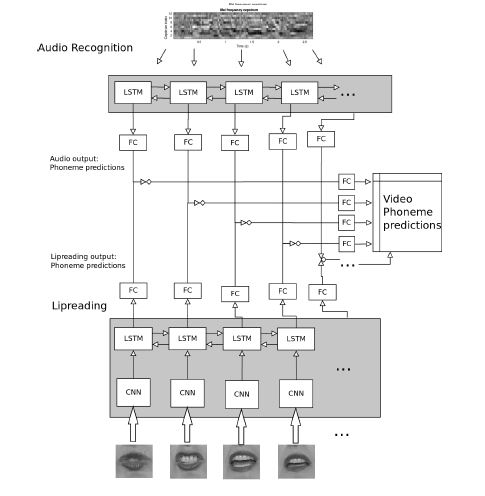
\includegraphics[width=0.3\textwidth]{Network Architecture.jpg}
\caption{\label{fig:Network Architecture}A brief network architecture employing audio-video ASR system is shown above.}
\end{figure}

The audio subnetwork takes in a sequence of MFCC features from each timeframe. The ’LSTM’ blocks represent the LSTM network at different timesteps. A ’timestep’ is a moment in time when a phoneme is spoken in a video. The LSTM processes the input sequence one frame at a time, but in two directions simultaneously (as it’s bidirectional, as the arrows show). The forward LSTM layers of the network process the sequencing front to back and the reverse LSTM layers process the sequence back to front. The FC classification layer processes the output at each timestep to generate phoneme predictions for each audio frame of the sequence. 
The video subnetwork takes in a sequence of images which is passed through CNN blocks which gives out selected features. The LSTM network processes the sequence formed by the outputs of the CNN for all of the images and does so in two directions (it’s a bidirectional network). The FC classification layer processes the output at each timestep to generate phoneme predictions for each image frame of the sequence. Outputs of both the networks are then combined and passed through a fully connected neural network to retrieve final video phoneme predictions.


\section{ARCHITECTURAL DETAILS}
\subsection{MFCC}
An important step to be able to train an audio recognizer is to divide the raw audio file in segments that can then be processed separately. A very common technique to do this is by using Mel-Frequency Cepstral Coefficients. MFCCs are the outputs of a cosine transformation of the logarithm of the short-term energy spectrum, expressed on a Mel-frequency scale. This scale takes into account human perception of sound, in contrast to a linear frequency scale. So they are a good way to express human speech information and are often used for speech recognition
MFCC coefficients are derived as follows:
\begin{enumerate}
\item Take the Fourier transform of (a windowed excerpt of) a signal.
\item Map the results to the Mel frequency scale with overlapping windows, and take a log of the powers at the Mel frequencies
\item Use these log powers as inputs for a discrete cosine transformation and keep the first 13 coefficients as MFCCs
\end{enumerate}

\subsection{FCNN}
Artificial Neural Networks are based on the structure of neurons in our own brains. They take some input values, perform a very simple operation on it, and pass their output to other neurons. In a Fully Connected Neural Networks (FCNN) each neuron is connected to every neuron in the previous layer, and each connection has its own weight. This type of networks has large amounts of weights and can learn complex relationships between inputs and outputs. These networks are hard to use for end-to-end classification as the network size explodes when the number of layers and the number of neurons per layer increases. Therefore they are often used after a feature extraction network. They further combine the features in some nonlinear way and classify them.
CNN: Convolutional Neural Networks (CNNs) have revolutionized image processing for many applications, especially for recognition and classification tasks. They are quite similar to normal FCNNs, but are organized in a different way.  Neurons connect only to a small part of the neurons in the previous layer, not to all of them. This reduces the number of network parameters enormously. CNNs are always multi-layered.
A CNN generally follows the structure shown below. It consists of convolutional (CONV) layers, nonlinearity layers (NonLin), pooling layers (POOL), and fully connected layers (FC).

Input− > [CONV − > NonLin− > POOL] *N− > [FC]*M− > FC(softmax)

A summary of the important properties of a CNN:
\begin{enumerate}
\item CONV layers convolve a number of filters across the height and width of the volume of neurons in the previous layer.
\item POOL layers to reduce the size of the data by downsampling along width and height. There are different types of pooling - Max Pooling, Average Pooling, and L2-Norm Pooling.
\item FC layers at the end perform classification
\end{enumerate}

Here, we intend to use 5 CONV layers with ReLu activations and 3 POOL layers performing max-pooling.

\subsection{LSTM}
Long Short-Term Memory Networks (LSTM) is a special kind of Recurrent Neural Networks, capable of learning long-term dependencies. An issue with standard feed-forward networks is that they can’t take into account time information. This is however extremely important for speech recognition. When a person has pronounced ’c’ and ’a’, the next letter might very well be an ’r’. The probability of it being ’t’ is quite low. LSTMs can use this time information by adding a kind of memory to the network in the form of internal states. 
Here, A 2 layer LSTM network with 256 units/layer will be deployed in the audio network and bi-directional 2 layer LSTM network with 256 units/layer will be deployed in the video network. Bidirectional LSTMs use the fact that the output at a certain time does not only depend on previous inputs but also future elements.


\section{COMPLEXITY ANALYSIS}
The computational complexity of the combined network is expected to be fairly low: the number of input features is limited to the sum of the number of output features from the audio and lipreading subnetworks. These correspond to the sizes of the last LSTM layers of those subnetworks, which are generally 512 or lower. The audio network and CNN are chosen to maintain a good balance between complexity and performance and is the same for all trained multimodal networks. CNNs require lots of computations. For CNN-based classifiers, over 90\% of the runtime is spent in the convolutional layers. Therefore most of the variation in complexity comes from the type of connections between the subnetwork. The use of raw features in all parts of the networks (lipreading CNN output, audio output, lipreading output) is expected to improve performance by a large margin but requires lots of weights for all of the connections. Weights in the CNN can be reused many times per image, and there’s one image for each timeframe. Audio LSTM weights will be used once per audio frame, of which there are more than one timeframes. Lipreading LSTM weights and weights in the FC combining layers will be used only once per time frame.  
Two main types of multimodal networks can be used. The first one using pre-classification after the CNN and the lipreading LSTM (but not after the audio LSTM). This means that the number of weights required to connect between the stages of the multimodal network will be limited as only the phoneme predictions are used as features. As inferred from the reference thesis, performance is expected to be quite high at 77.55\%. The second type does not use any pre-classification. It achieves 76.19\% for clean audio. If trained end-to-end, it achieves the highest score of all trained networks for clean audio (81.10\%) but does not perform well for noisy audio (31.17\%). It requires a lot more connection weights than the network with pre-classification. If trained with an attention network, it does perform very well under noisy conditions (58.55\%).


\section{DATASET AND TRAINING}
Training will be done using TCD-TIMIT audiovisual dataset. It consists of 13826 video clips in MP4 format of 62 speakers reading a total of 6913 sentences from the TIMIT corpus. The TCD-TIMIT are mostly volunteers, both males and females. The dataset also includes three professional lip-speakers, who each speak 377 sentences. Top-1 classification accuracy and Top-3 accuracy will be used as a measure of performance. 
To further evaluate the performance, the multimodal network can be trained in two ways: the first one using ’fixed subnetworks’, meaning that the weights of the lipreading and audio networks will be fixed during training of the combined network. As a result of this, only the weights of the FC combination layers will be trained. The second way will be to train all of the weights of the multimodal network, also the weights of the lipreading and audio networks. This will be referred to as End-to-End Training.


\section{EXISTING CODEBASE}
The reference thesis has existing work on the multimodalSR Lip Reading in Lasagne. We will be rewriting the code from scratch in Keras and will work on implementing End-to-End Network with Attention Network which is not present in the existing codebase. 


\section{MAJOR CHALLENGES}
The networks will be trained and evaluated on clean, noise-free audio. However, In a real-world situation, the audio will not be noise-free. So, When noise is added to the audio data, the performance of the audio network is expected to decreases sharply. An explanation could be that the multimodal network relies more on the audio than on the lipreading (since audio-only recognition performance is usually better than lipreading-only performance). 
To overcome this challenge, we intend to add an attention network (AN) that decides the relative importance of the visual-only and audio-only outputs. Attention networks are fully connected networks somewhat separate from the normal network structure. The audio-only output features and lipreading-only output features will be provided as inputs to the AN. When audio quality is high, the audio network will produce one feature with a much higher value than the others. The AN will notice this, and the relative weights for the audio network will be high. The lipreading network will also provide predictions, but the values will be more ’spread out’ as it will not be as accurate as the audio network. The AN will notice this, and the weights for the lipreading network features will be lower than those for the audio network features


\section{FINAL TEST SET-UP}
The trained network will be evaluated on the test set of TCD-TIMIT (containing only volunteers). The test set is constructed in such a way that no speaker will have videos in both training and test set. This is done to evaluate the generalization capability of the model, i.e to make sure that the model is not speaker dependent. For performance measurement classification tasks, top-k accuracy will be used as a metric. For each input sample, the k predictions of the network with the highest probability score are compared with the real label. If one of those k predictions is correct, the evaluation is counted as correct. If not, it is counted as wrong. The final top-k accuracy score is then the fraction of samples that were predicted correctly compared to the total number of input samples.



\section{ROUGH TIMELINE}
The work will be split into groups as per below. Once individual modules are complete, the network will be combined and tested end-to-end. Possibility of doing Audio Network and Lip Reading Network simultaneously by dividing the task among us will also be explored.
\begin{enumerate}
\item Audio Network: Involves MFCC and training LSTM, FCNN for audio to phoneme prediction. - 1 Week
\item Lipreading Network: Involves training CNNs, LSTMs, FCNN for image sequence to phoneme prediction. - 1 Week
\item Combined FCNN: Training FCNN for synchronized prediction from audio and video modules for greater accuracy. - 1 Week
\item Testing: Testing on the end-to-end model for overall accuracy. - 2 days
\item Attention Networks: Modifying our design to include Attention Based Networks, and re-train to improve accuracy even further. - 3 Weeks
\item Testing the model with Attention Networks: 3 days
\end{enumerate}


\section{REFERENCES}
\begin{enumerate}
\item J. S. Chung, A. Senior, O. Vinyals, and A. Zisserman, “Lip reading sentences in the wild,” arXiv preprint arXiv:1611.05358, 2016.
\item K. Noda, Y. Yamaguchi, K. Nakadai, H. G. Okuno, and T. Ogata, “Lipreading using the convolutional neural network.” 2014.
\item Amit Garg, Jonathan Noyala and Sameep Bagadia, “Lip reading using CNN and LSTM” , 2016
\item M. Wand, J. Koutnk, and J. Schmidhuber, “Lipreading with long short-term memory,” 2016.
\item Matthijs Van keirsbilck, “Design, implementation, and analysis of a deep convolutional-recurrent neural network for speech recognition through audiovisual sensor fusion.”, KU Leuven, 2016 – 2017.
\item “Multimodal speech recognition using lipreading (with CNNs) and audio (using LSTMs)” https://github.com/matthijsvk/multimodalSR
\end{enumerate}



\bibliographystyle{plain}
\bibliography{references.bib}


\end{document}
